\section{Desarrollo}

\subsection{Preparación del Entorno y Estado Inicial de la Red}
Para la realización de esta práctica, se utilizó la herramienta de simulación Cisco Packet Tracer. Se partió del archivo base proporcionado (\texttt{IPsecVPN.pka}), el cual ya cuenta con la topología estructurada y las direcciones IP estáticas previamente configuradas tanto en los dispositivos finales como en los routers.

\begin{figure}[H]
        \centering
        \fbox{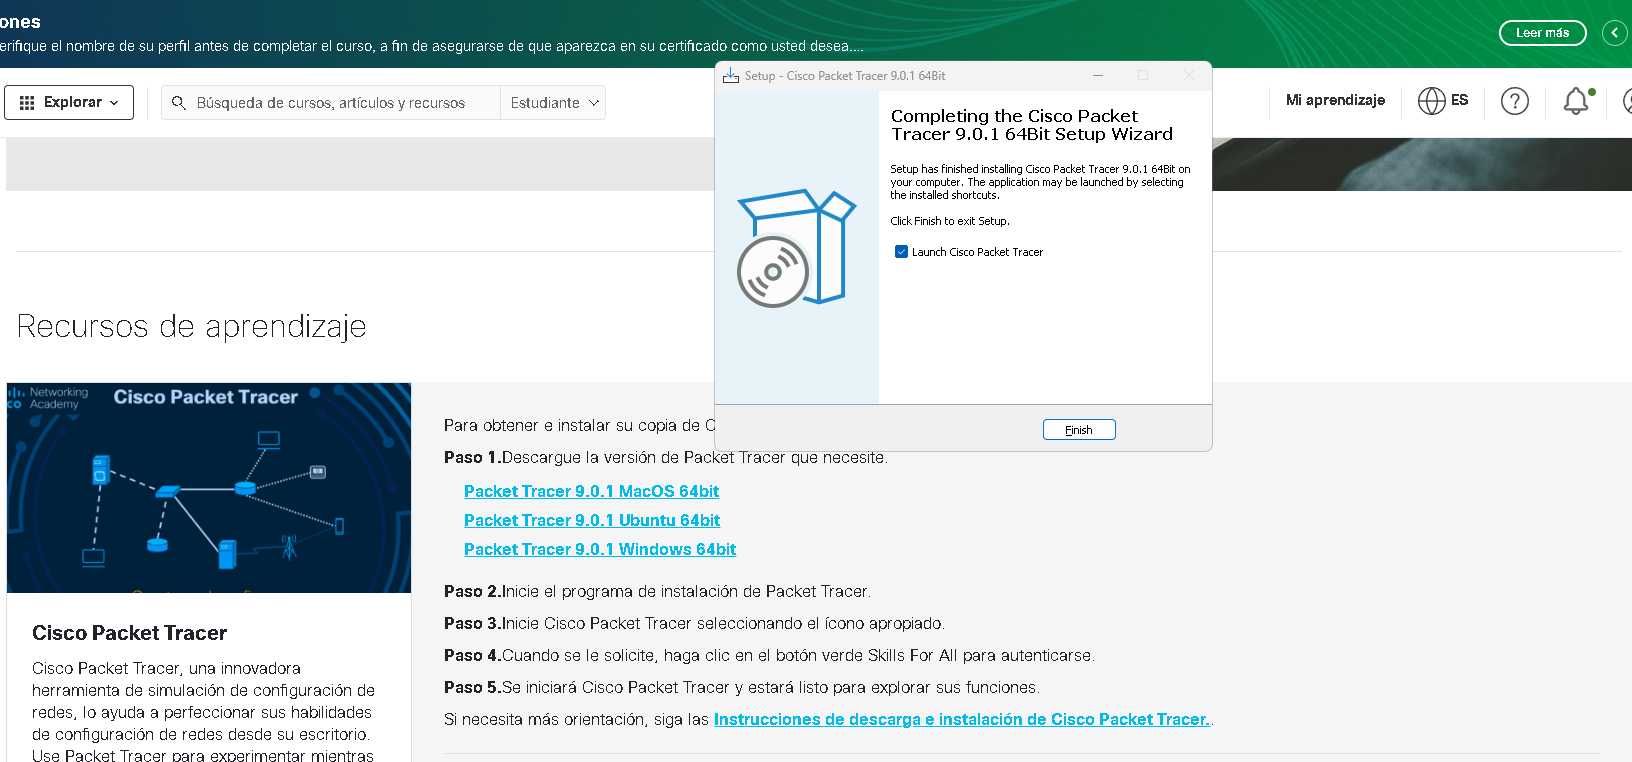
\includegraphics[width=0.9\textwidth]{Imagenes/Instalacion.png}}
        \caption{Descarga e instalación de Cisco Packet Tracer.}
        \label{fig:instalacion-pt}
\end{figure}

Descargamos de la página oficial de Cisco la versión 9.0.1 de Packet Tracer (Windows en nuestro caso) y procedimos a instalarla siguiendo los pasos del ejecutable. Una vez finalizada la instalación, se ejecutó el programa.

\begin{figure}[H]
        \centering
        \fbox{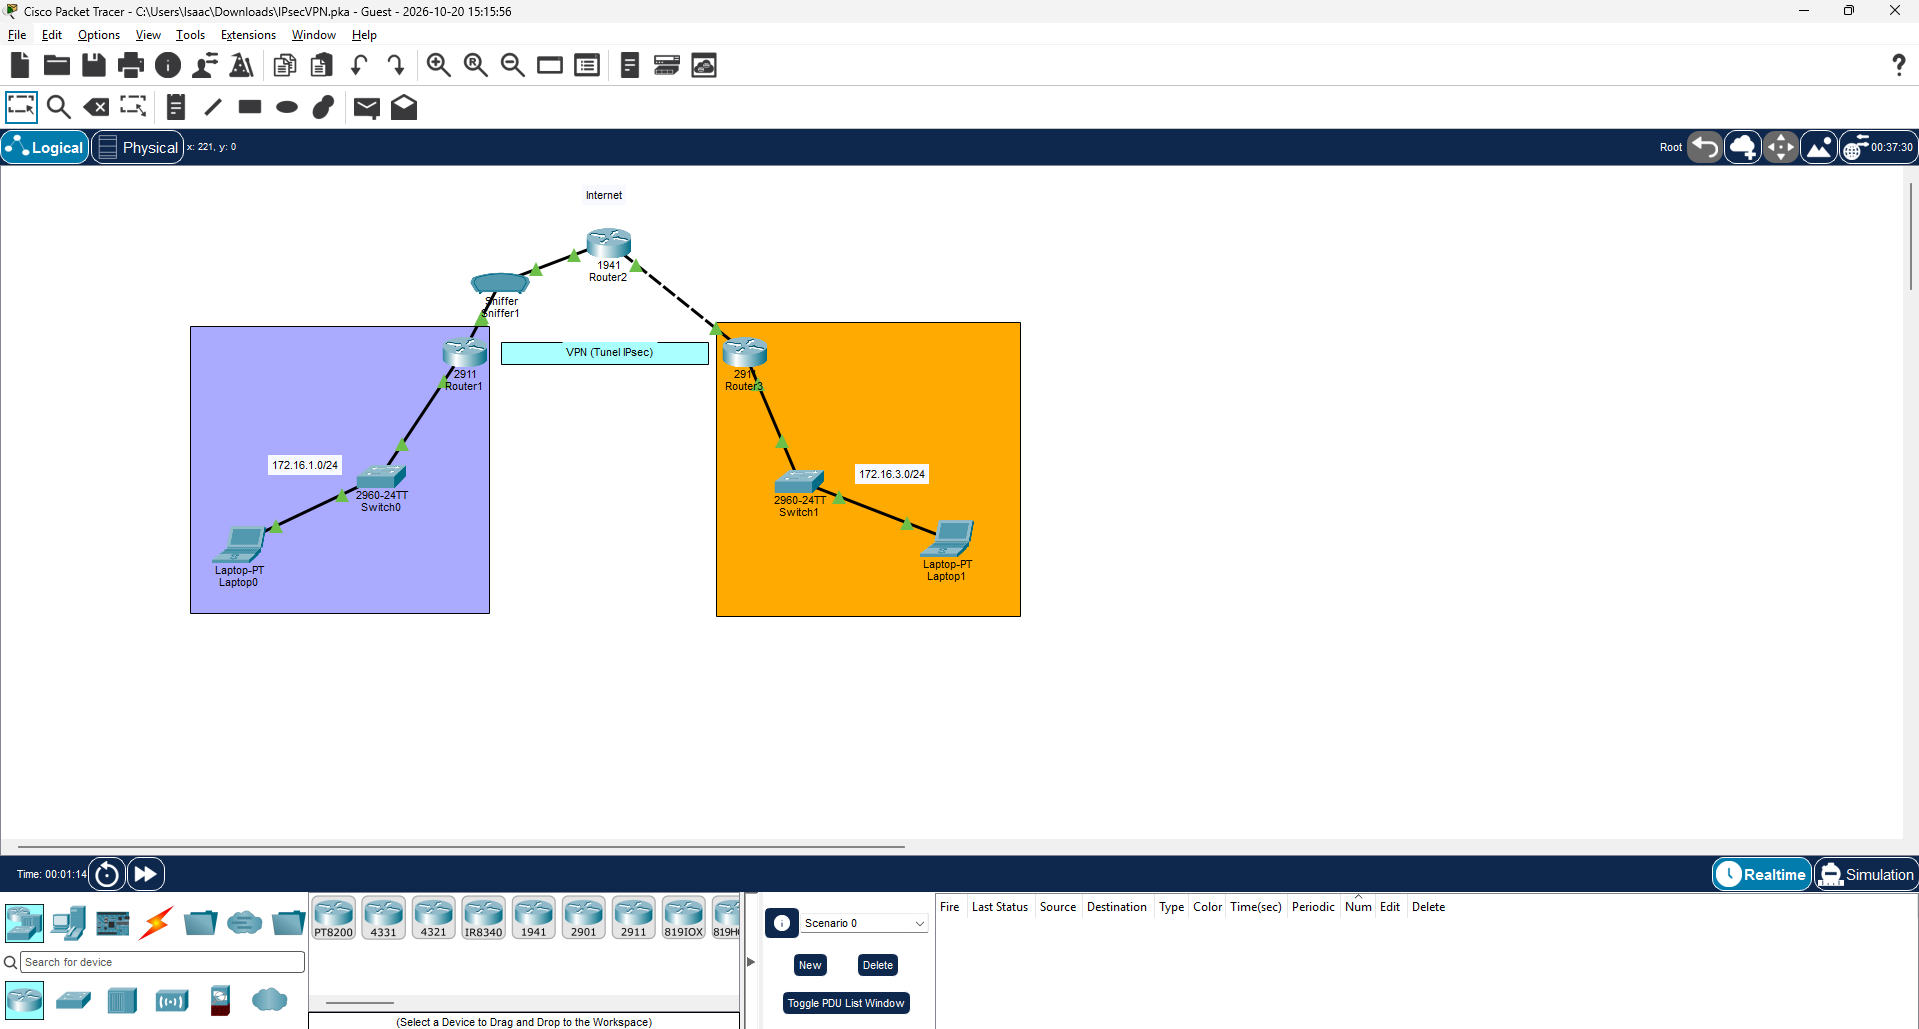
\includegraphics[width=0.9\textwidth]{Imagenes/cargar.png}}
        \caption{Carga del archivo IPsecVPN.pka y vista de la topología.}
        \label{fig:carga-archivo}
\end{figure}

Como se observa en la topología, ya cuenta con el dispositivo intermedio llamado \textbf{Sniffer1}, el cual está conectado físicamente en el enlace entre el \texttt{Router1} y el \texttt{Router2} (este último simulando la red de Internet). Este dispositivo nos permitirá auditar e inspeccionar los paquetes que viajan a través del enlace público.

\subsection{Inspección de Tráfico sin Cifrar (Antes de IPsec)}
Antes de configurar los túneles VPN, se procedió a verificar la conectividad de extremo a extremo y a analizar el estado de los datos en tránsito. Desde la consola de comandos de la \texttt{Laptop0} (ubicada en la red local 172.16.1.0/24), se ejecutó un comando \texttt{ping} dirigido a la \texttt{Laptop1} (con dirección IP 172.16.3.100).

Al revisar el tráfico capturado por el \texttt{Sniffer1} durante esta prueba de conectividad, se pudo constatar que los paquetes viajaban utilizando el protocolo \textbf{ICMP} en texto claro. Esto demuestra de manera práctica que, sin la implementación de una VPN, la información es completamente vulnerable a ser interceptada en su trayecto por la red pública.

\begin{figure}[H]
    \centering
    \fbox{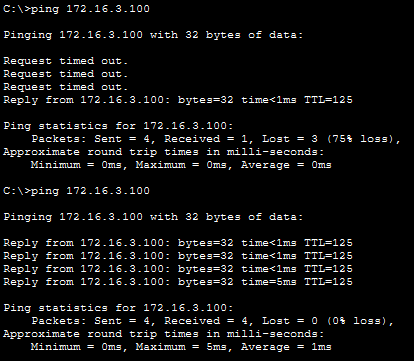
\includegraphics[width=0.9\textwidth]{Imagenes/ping.png}}
    \caption{Prueba de conectividad exitosa entre \texttt{Laptop0} y \texttt{Laptop1}.}
    \label{fig:ping-sin-cifrar}
\end{figure}

Como se puede observar en la figura \ref{fig:ping-sin-cifrar}, en un primer intento de ejecutar el \texttt{ping}, tuvimos un tiempo de espera agotado (\texttt{Request timed out}) de 3 paquetes, tal vez debido a que los routers aún no habían establecido la ruta de retorno. Sin embargo, en el segundo intento, los paquetes fueron respondidos y recibidos exitosamente, evidenciando que la conectividad entre los extremos de la red es funcional.

\begin{figure}[H]
    \centering
    \fbox{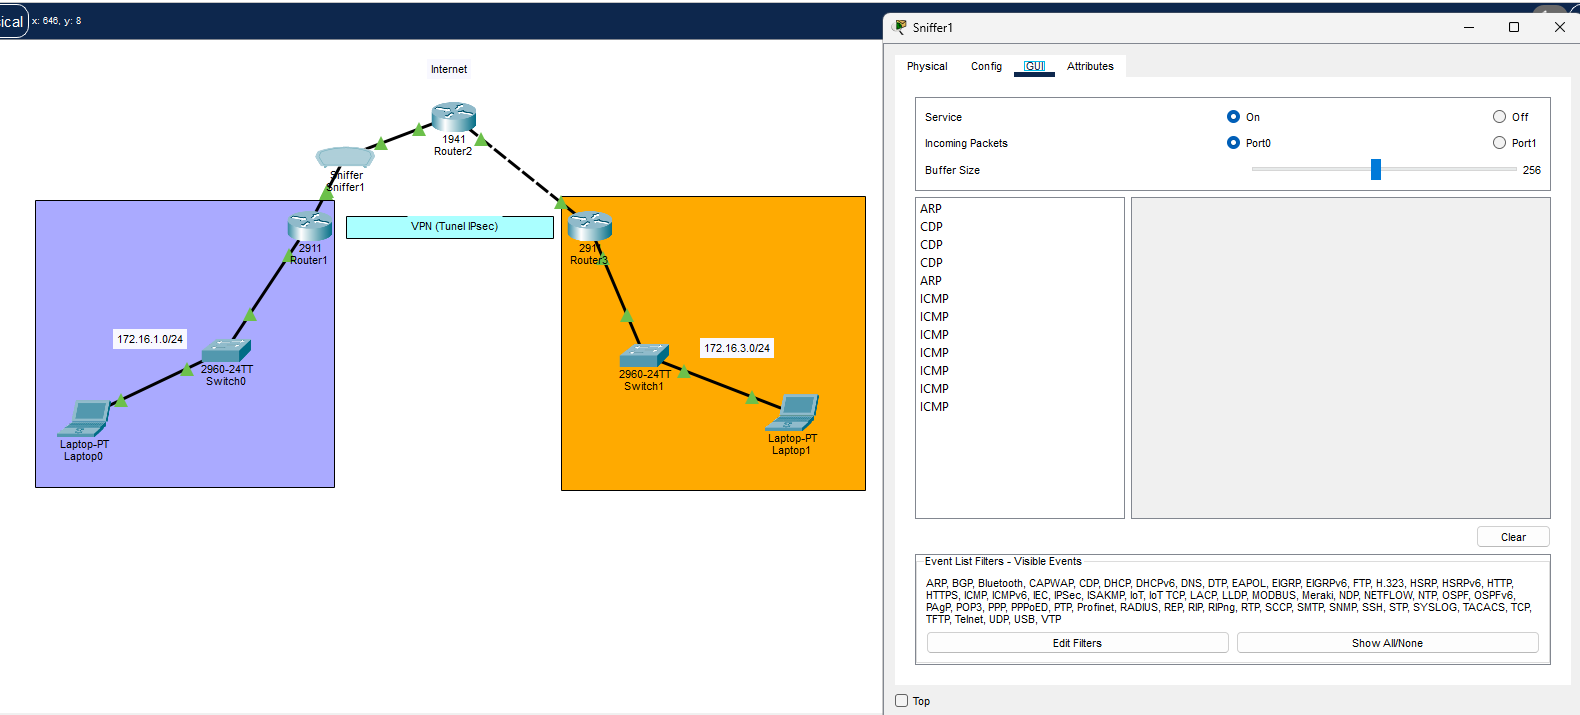
\includegraphics[width=0.9\textwidth]{Imagenes/sniffer.png}}
    \caption{Captura del Sniffer evidenciando tráfico ICMP sin cifrar.}
    \label{fig:tráfico-sin-cifrar}
\end{figure}

\subsection{Activación de la Licencia de Seguridad (securityk9)}
Para poder implementar la suite de protocolos IPsec y configurar los parámetros del túnel VPN, tuvimos que habilitar las funciones criptográficas en los routers que fungirán como extremos del túnel (\texttt{R\_01} y \texttt{R\_03}). 

Debido a que el hardware simulado en esta topología corresponde a la familia de routers Cisco 2911, se procedió a activar la licencia específica del módulo \texttt{c2900}. Esto se logró ingresando al modo de configuración global y ejecutando el comando \texttt{license boot module c2900 technology-package securityk9}. 

Durante este proceso, el sistema solicitó leer y aceptar el acuerdo de licencia de usuario final (EULA), a lo cual se respondió afirmativamente (\texttt{yes}). Posteriormente, se procedió a reiniciar el equipo mediante el comando \texttt{reload} para que los cambios surtieran efecto en el sistema operativo del router.

Ejecutamos el siguiente conjunto de comandos en ambos routers para habilitar la licencia y reiniciar el sistema:
\begin{lstlisting}[language=]
Router> enable
Router# show version
Router# configure terminal
Router(config)# license boot module c2900 technology-package securityk9
Router(config)# exit
Router# copy run start startup-config
Router# reload
Router# show version
\end{lstlisting}

\begin{figure}[H]
        \centering
        \fbox{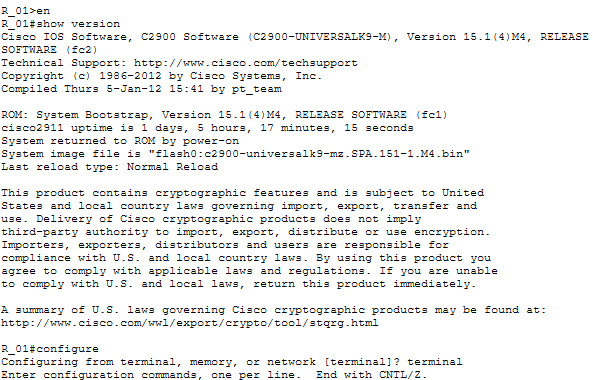
\includegraphics[width=0.9\textwidth]{Imagenes/config.png}}
        \caption{Ingreso al modo de configuración y revisión inicial de versión.}
        \label{fig:ingreso-configuracion}
\end{figure}

\begin{figure}[H]
        \centering
        \fbox{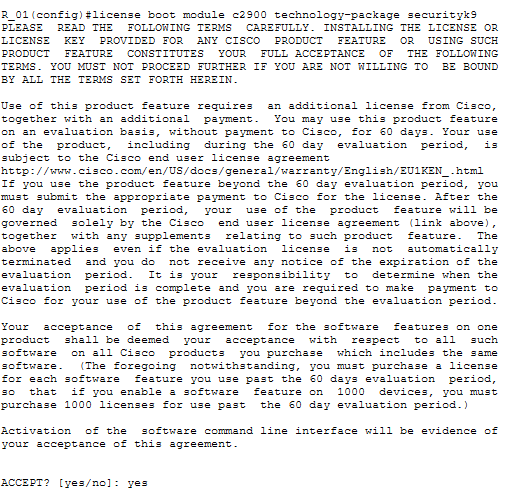
\includegraphics[width=0.9\textwidth]{Imagenes/licencia.png}}
        \caption{Activación de la licencia y aceptación de los términos de Cisco.}
        \label{fig:activacion-licencia}
\end{figure}
    
\begin{figure}[H]    
        \centering
        \fbox{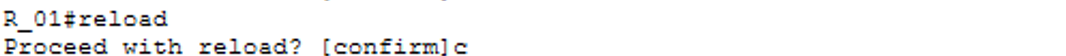
\includegraphics[width=0.9\textwidth]{Imagenes/reinicio.png}}
        \caption{Reinicio del router (\texttt{reload}) presionando enter para confirmar.}
        \label{fig:reinicio-router}
\end{figure}

En este punto de la práctica, los equipos se reiniciaron exitosamente. Tras el arranque, nos aseguramos de que todo estuviera funcionando correctamente y se ejecutó el comando \texttt{show version} verificando que el paquete \texttt{securityk9} ahora se encuentra activo (a comparación con la versión anterior que se encontraba inactiva), lo que permite el uso de comandos criptográficos en el sistema.

\begin{figure}[H]
        \centering
        \fbox{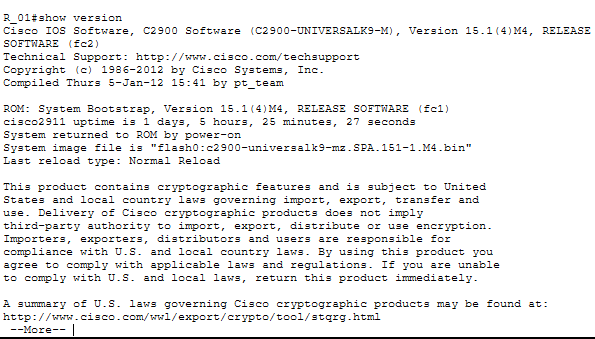
\includegraphics[width=\linewidth]{Imagenes/showversion.png}}
        \caption{Comando \texttt{show version} ejecutado tras el reinicio en \texttt{R\_01}.}
        \label{fig:show-version}
\end{figure}

\begin{figure}[H]
        \centering
        \fbox{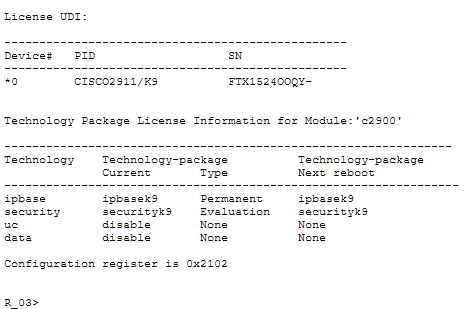
\includegraphics[width=\linewidth]{Imagenes/verificacion.png}}
        \caption{Verificación exitosa del estado activo de la licencia \texttt{securityk9}.}
        \label{fig:verificacion-licencia}
\end{figure}

Realizamos este mismo procedimiento tanto para el router \texttt{R\_01} como para el router \texttt{R\_03}, asegurando que ambos extremos del túnel VPN estén correctamente habilitados para soportar la suite de protocolos IPsec.

\subsection{Configuración de la Lista de Control de Acceso (ACL)}
Una vez habilitadas las licencias, el primer paso lógico para establecer el túnel fue definir el "tráfico interesante", es decir, establecer qué flujo de datos debe ser capturado por la VPN para ser cifrado. 

Para lograr esto, se configuró una Lista de Control de Acceso Extendida (ACL 100) en ambos routers. En \texttt{R\_01}, se permitió el tráfico desde la red origen 172.16.1.0/24 hacia la red destino 172.16.3.0/24. De manera simétrica, en \texttt{R\_03} se configuró la regla inversa, permitiendo el tráfico desde 172.16.3.0/24 hacia 172.16.1.0/24.

Ejecutamos para R\_01:

\begin{lstlisting}[language=]
    R_01(config)# access-list 100 permit ip 172.16.1.0 0.0.0.255 172.16.3.0 0.0.0.255
\end{lstlisting}

Y para R\_03:
\begin{lstlisting}[language=]
    R_03(config)# access-list 100 permit ip 172.16.3.0 0.0.0.255 172.16.1.0 0.0.0.255
\end{lstlisting}

\begin{figure}[H]
    \centering
    \fbox{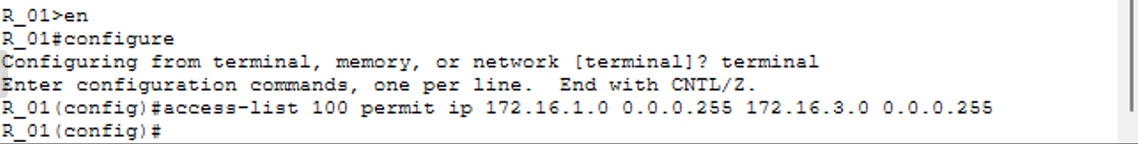
\includegraphics[width=0.9\textwidth]{Imagenes/ACL1.png}}
    \fbox{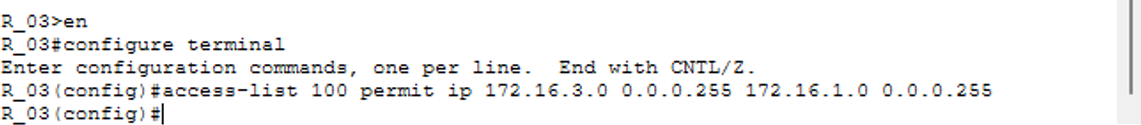
\includegraphics[width=0.9\textwidth]{Imagenes/ACL2.png}}
    \caption{Configuración de las ACL simétricas para definir el tráfico interesante en ambos routers.}
    \label{fig:configuracion-acl}
\end{figure}

\subsection{Configuración de la Fase 1 del Túnel (ISAKMP SA)}
Con el tráfico definido, se procedió a configurar la Fase 1, cuyo objetivo es establecer un canal de gestión seguro y autenticado entre los routers antes de negociar los parámetros de los datos.

Se creó la política ISAKMP (política 10) definiendo los siguientes atributos (HAGLE):
\begin{itemize}
    \item \textbf{Cifrado (Encryption):} AES-256 para asegurar la confidencialidad de la gestión.
    \item \textbf{Hash:} MD5 para la verificación de integridad de los mensajes.
    \item \textbf{Autenticación:} Clave pre-compartida (\texttt{pre-share}).
    \item \textbf{Grupo Diffie-Hellman:} Grupo 5, para establecer el nivel de seguridad del intercambio de claves.
    \item \textbf{Tiempo de vida (Lifetime):} 86400 segundos (24 horas) para la validez de la sesión.
\end{itemize}

Posteriormente, se configuró la llave pre-compartida (\texttt{VPNpass}), indicándole a cada router la dirección IP pública de su vecino (peer) correspondiente para establecer el vínculo.

\begin{figure}[H]
    \centering
    \begin{minipage}{0.48\textwidth}
        \centering
        \fbox{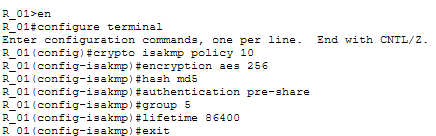
\includegraphics[width=0.9\textwidth]{Imagenes/r11.png}}
        \fbox{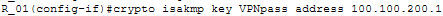
\includegraphics[width=0.9\textwidth]{Imagenes/r12.png}}
        \caption{Configuración de los parámetros ISAKMP (Fase 1) en \texttt{R\_01}.}
        \label{fig:configuracion-isakmp-r1}
    \end{minipage}\hfill
    \begin{minipage}{0.48\textwidth}
        \centering
        \fbox{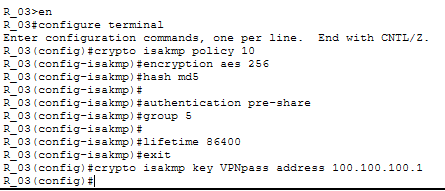
\includegraphics[width=0.9\textwidth]{Imagenes/r31.png}}
        \caption{Configuración equivalente de los parámetros ISAKMP en \texttt{R\_03}.}
        \label{fig:configuracion-isakmp-r3}
    \end{minipage}
\end{figure}

\subsection{Configuración de la Fase 2 y Crypto Map}
La etapa final consistió en definir cómo se protegerían los datos de los usuarios (Fase 2). Para ello, se creó un \texttt{transform-set} que emplea \texttt{esp-aes 256} para cifrar el contenido del paquete y \texttt{esp-sha-hmac} para autenticar los datos. 

Finalmente, se vinculó la política de Fase 1, la Fase 2 y la ACL a través de un Mapa Criptográfico (\texttt{crypto map IPSEC-CRYPTOMAP}). Este mapa se aplicó directamente a la interfaz de salida de cada router hacia Internet (\texttt{GigabitEthernet0/0}), lo cual disparó un mensaje de confirmación del sistema indicando que el protocolo ISAKMP quedó activo en la interfaz.

Ejecutamos los comandos en \texttt{R\_01}:
\begin{lstlisting}[language=]
    R_01(config)# crypto ipsec transform-set R_01-R_03 esp-aes 256 esp-sha-hmac
    R_01(config)# crypto map IPSEC-CRYPTOMAP 100 ipsec-isakmp
    R_01(config-crypto-map)# set peer 100.100.200.1
    R_01(config-crypto-map)# set pfs group5
    R_01(config-crypto-map)# set security-association lifetime seconds 86400
    R_01(config-crypto-map)# set transform-set R_01-R_03
    R_01(config-crypto-map)# match address 100
    R_01(config-crypto-map)# exit
    R_01(config)# interface GigabitEthernet0/0
    R_01(config-if)# crypto map IPSEC-CRYPTOMAP
\end{lstlisting}

Análogamente, en \texttt{R\_03} se ejecutaron los mismos anteriores comandos, solo que cambiando la dirección IP del peer a \texttt{100.100.100.1} y el nombre del \texttt{transform-set} a \texttt{R\_03-R\_01}.

\begin{figure}[H]
    \centering
    \begin{minipage}{0.48\textwidth}
        \centering
        \fbox{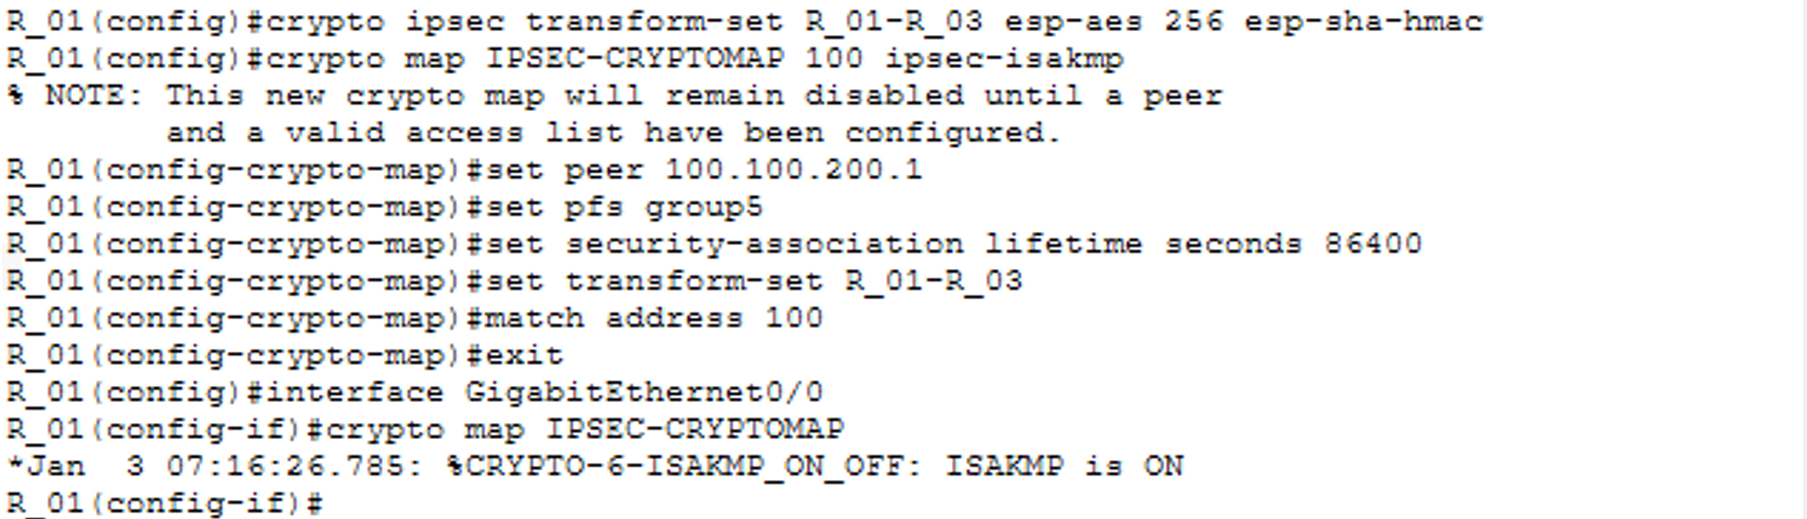
\includegraphics[width=1\textwidth]{Imagenes/ISAKMP1.png}}
        \caption{Creación del Crypto Map en \texttt{R\_01} y su aplicación a la interfaz de salida WAN.}
        \label{fig:crypto-map-r1}
    \end{minipage}
    \begin{minipage}{0.48\textwidth}
        \centering
        \fbox{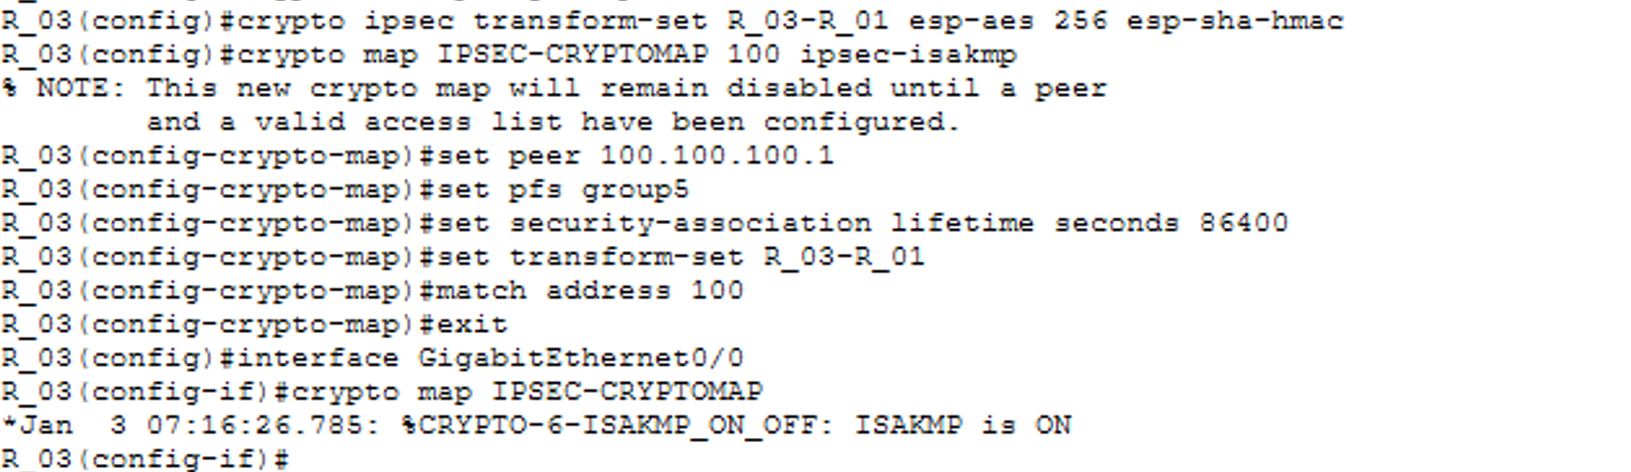
\includegraphics[width=1\textwidth]{Imagenes/ISAKMP2.png}}
        \caption{Creación del Crypto Map en \texttt{R\_03} y su aplicación a la interfaz de salida WAN.}
        \label{fig:crypto-map-r3}
    \end{minipage}
\end{figure}

\subsection{Verificación del Funcionamiento del Túnel VPN}
Para corroborar que el túnel IPSec se estableció correctamente y está cifrando los datos, se procedió a realizar una nueva prueba de conectividad mediante comandos \texttt{ping} desde la \texttt{Laptop0} hacia la \texttt{Laptop1}. Al principio, nuevamente obtuvimos "Request timed out" mientras los routers establecen el túnel, pero al segundo intento, los paquetes subsecuentes se transmitieron de manera exitosa.

\begin{figure}[H]
    \centering
    \fbox{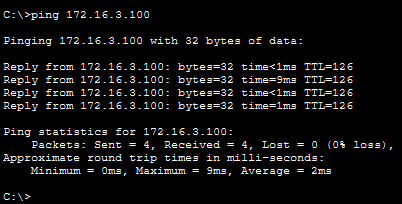
\includegraphics[width=0.6\textwidth]{Imagenes/pingvpn.png}}
    \caption{Nuevo envío de paquetes ICMP tras configurar la VPN; el tiempo de respuesta se estabiliza tras la negociación.}
    \label{fig:ping-con-vpn}
\end{figure}

Al inspeccionar nuevamente el dispositivo \texttt{Sniffer1} ubicado en el enlace público, el comportamiento del tráfico cambió drásticamente respecto a la prueba inicial. En lugar de registrar el protocolo ICMP en texto claro, el sniffer capturó primero los paquetes \textbf{ISAKMP} correspondientes a la negociación de llaves (Fase 1), seguidos inmediatamente por el tráfico \textbf{IPSec} cifrando la carga útil (ESP), demostrando que la Fase 2 está activa y protegiendo el contenido del \texttt{ping}.

\begin{figure}[H]
    \centering
    \fbox{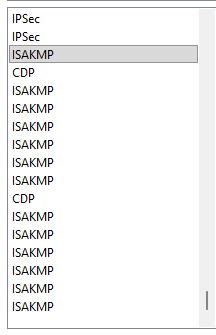
\includegraphics[width=0.3\textwidth]{Imagenes/sniffervpn.png}}
    \caption{Sniffer capturando tráfico ISAKMP (negociación) e IPSec (datos cifrados).}
    \label{fig:sniffer-vpn}
\end{figure}

Finalmente, como verificación a nivel de consola, se ejecutó el comando \texttt{show crypto ipsec sa} en los routers extremos. La salida arrojó el funcionamiento de la VPN: en \texttt{R\_01} se observaron los contadores incrementados (\texttt{\#pkts encrypt: 6}, \texttt{\#pkts decrypt: 5}), confirmando que los paquetes están siendo procesados por el motor criptográfico. Asimismo, se comprobó el uso de las direcciones IP públicas correctas en los \texttt{crypto endpt} locales y remotos, y el \texttt{Status: ACTIVE} del túnel ESP, validando así el éxito total de la práctica.

La salida del comando en \texttt{R\_01} fue la siguiente:
\begin{lstlisting}[language=]
R_01#show crypto ipsec sa
interface: GigabitEthernet0/0
Crypto map tag: IPSEC-CRYPTOMAP, local addr 100.100.100.1
protected vrf: (none)
local ident (addr/mask/prot/port): (172.16.1.0/255.255.255.0/0/0)
remote ident (addr/mask/prot/port): (172.16.3.0/255.255.255.0/0/0)
current_peer 100.100.200.1 port 500
PERMIT, flags={origin_is_acl,}
#pkts encaps: 6, #pkts encrypt: 6, #pkts digest: 0
#pkts decaps: 5, #pkts decrypt: 5, #pkts verify: 0
#pkts compressed: 0, #pkts decompressed: 0
#pkts not compressed: 0, #pkts compr. failed: 0
#pkts not decompressed: 0, #pkts decompress failed: 0
#send errors 1, #recv errors 0
local crypto endpt.: 100.100.100.1, remote crypto endpt.:100.100.200.1
path mtu 1500, ip mtu 1500, ip mtu idb GigabitEthernet0/0
current outbound spi: 0xC36CBF65(3278684005)
inbound esp sas:
spi: 0x5BF65BCB(1542872011)
transform: esp-aes 256 esp-sha-hmac ,
in use settings ={Tunnel, }
conn id: 2005, flow_id: FPGA:1, crypto map: IPSEC-CRYPTOMAP
sa timing: remaining key lifetime (k/sec): (4525504/86105)
IV size: 16 bytes
replay detection support: N
Status: ACTIVE
inbound ah sas:
inbound pcp sas:
outbound esp sas:
spi: 0xC36CBF65(3278684005)
transform: esp-aes 256 esp-sha-hmac ,
in use settings ={Tunnel, }
conn id: 2006, flow_id: FPGA:1, crypto map: IPSEC-CRYPTOMAP
sa timing: remaining key lifetime (k/sec): (4525504/86105)
IV size: 16 bytes
replay detection support: N
Status: ACTIVE
outbound ah sas:
outbound pcp sas:
\end{lstlisting}

Y la salida del comando en \texttt{R\_03} fue la siguiente:
\begin{lstlisting}[language=]
R_03#show crypto ipsec sa
interface: GigabitEthernet0/0
Crypto map tag: IPSEC-CRYPTOMAP, local addr 100.100.200.1
protected vrf: (none)
local ident (addr/mask/prot/port): (172.16.3.0/255.255.255.0/0/0)
remote ident (addr/mask/prot/port): (172.16.1.0/255.255.255.0/0/0)
current_peer 100.100.100.1 port 500
PERMIT, flags={origin_is_acl,}
#pkts encaps: 5, #pkts encrypt: 5, #pkts digest: 0
#pkts decaps: 6, #pkts decrypt: 6, #pkts verify: 0
#pkts compressed: 0, #pkts decompressed: 0
#pkts not compressed: 0, #pkts compr. failed: 0
#pkts not decompressed: 0, #pkts decompress failed: 0
#send errors 0, #recv errors 0
local crypto endpt.: 100.100.200.1, remote crypto endpt.:100.100.100.1
path mtu 1500, ip mtu 1500, ip mtu idb GigabitEthernet0/0
current outbound spi: 0x5BF65BCB(1542872011)
inbound esp sas:
spi: 0xC36CBF65(3278684005)
transform: esp-aes 256 esp-sha-hmac ,
in use settings ={Tunnel, }
conn id: 2005, flow_id: FPGA:1, crypto map: IPSEC-CRYPTOMAP
sa timing: remaining key lifetime (k/sec): (4525504/86081)
IV size: 16 bytes
replay detection support: N
Status: ACTIVE
inbound ah sas:
inbound pcp sas:
outbound esp sas:
spi: 0x5BF65BCB(1542872011)
transform: esp-aes 256 esp-sha-hmac ,
in use settings ={Tunnel, }
conn id: 2006, flow_id: FPGA:1, crypto map: IPSEC-CRYPTOMAP
sa timing: remaining key lifetime (k/sec): (4525504/86081)
IV size: 16 bytes
replay detection support: N
Status: ACTIVE
outbound ah sas:
outbound pcp sas:
\end{lstlisting}

Dando por terminada la parte práctica, se concluye que la VPN IPSec fue configurada correctamente y está funcionando como se esperaba, asegurando la confidencialidad e integridad de los datos transmitidos entre las dos redes locales a través del enlace público.